\documentclass[14pt,a4paper]{extarticle}
\usepackage{extsizes}
\usepackage{cmap} % для кодировки шрифтов в pdf
%\documentclass[a4paper,12pt]{article} %размер бумаги устанавливаем А4, шрифт 12пунктов
\usepackage[utf8]{inputenc}%включаем свою кодировку: koi8-r или utf8 в UNIX, cp1251 в Windows
\usepackage[T2A, T1]{fontenc}
\usepackage[english,russian]{babel}%используем русский и английский языки с переносами
\usepackage{amssymb,amsfonts,amsmath,mathtext,cite,enumerate,amsthm,mathenv} %подключаем нужные пакеты расширений
\numberwithin{equation}{section}
\usepackage{graphicx} %хотим вставлять в диплом рисунки?
\usepackage{indentfirst} % Красная строка
\graphicspath{{images/}}%путь к рисункам
\usepackage{hyperref}
\usepackage{framed}
\usepackage{color} %% это для отображения цвета в коде
\usepackage{listings} %% собственно, это и есть пакет listingsb
\usepackage{ucs}
\usepackage{latexsym}
\usepackage{bm}
\usepackage{array}
\usepackage{multirow}
\usepackage{ulem}
\usepackage{csvsimple}

\frenchspacing
%----------------ЗАГОЛОВКИ---------------------------
\usepackage{titlesec}

\titleformat{\chapter}[display]
    {\filcenter}
    {\MakeUppercase{\chaptertitlename} \thechapter}
    {8pt}
    {\bfseries}{}
 
\titleformat{\section}
    {\centering\normalsize\bfseries}
    {\thesection}
    {1em}{\MakeUppercase}
 
\titleformat{\subsection}
    {\normalsize\bfseries}
    {\thesubsection}
    {1em}{}

% Настройка вертикальных и горизонтальных отступов
%\titlespacing*{\chapter}{0pt}{-30pt}{8pt}
\titlespacing*{\section}{\parindent}{*4}{*4}
\titlespacing*{\subsection}{\parindent}{*4}{*4}
%------------------------------------------------------

%---------------------ПОЛЯ-----------------------------
\usepackage{geometry}
\geometry{left=3cm}
\geometry{right=1.5cm}
\geometry{top=2.4cm}
\geometry{bottom=2.4cm}


\makeatletter
\renewcommand{\@biblabel}[1]{#1.} % Заменяем библиографию с квадратных скобок на точку:
\makeatother

\makeatletter


\def\x@multispan#1{%
  \global\let\@tempa\@empty
  \@multicnt#1\relax
  \loop\ifnum\@multicnt>\@ne
  \xdef\@tempa{\@tempa\kern\dimen@i\hfill&\omit}%
   \advance\@multicnt\m@ne
  \repeat
  \@tempa\kern\dimen@i\hfill}


\long\def\xmulticolumn#1#2#3{%
 \omit
 \begingroup
   \def\@addamp{\if@firstamp \@firstampfalse \else
                \@preamerr 5\fi}%
  \@mkpream{#2}\@addtopreamble\@empty
  \endgroup
  \def\@sharp{#3}%
  \setbox\z@\hbox{{\@preamble}}%
\global\dimen@i\wd\z@
\global\divide\dimen@i#1\relax
 \ignorespaces
\x@multispan{#1}}
\makeatother

\linespread{1.5} % полуторный интервал
%\renewcommand{\baselinestretch}{1.5}
\renewcommand{\theenumi}{\arabic{enumi}}% Меняем везде перечисления на цифра.цифра
\renewcommand{\labelenumi}{\arabic{enumi}}% Меняем везде перечисления на цифра.цифра
\renewcommand{\theenumii}{.\arabic{enumii}}% Меняем везде перечисления на цифра.цифра
\renewcommand{\labelenumii}{\arabic{enumi}.\arabic{enumii}.}% Меняем везде перечисления на цифра.цифра
\renewcommand{\theenumiii}{.\arabic{enumiii}}% Меняем везде перечисления на цифра.цифра
\renewcommand{\labelenumiii}{\arabic{enumi}.\arabic{enumii}.\arabic{enumiii}.}% Меняем везде перечисления на цифра.цифра
%\renewcommand{\figurename}{Рисунок} 
\addto\captionsrussian{
\def\figurename{Рисунок}
\renewcommand{\refname}
    {Список использованных источников}
}
\usepackage[labelsep=space]{caption}
\DeclareCaptionLabelSeparator{bar}{ - }
\captionsetup{
  labelsep=bar
}

\usepackage{floatrow}
\DeclareFloatFont{tiny}{\tiny}
\floatsetup[table]{font=footnotesize,capposition=top}

%\usepackage{sectsty}

%\allsectionsfont{\centering}


\lstset{ %
language=Python,                 % выбор языка для подсветки (здесь это Python)
basicstyle=\scriptsize\sffamily, % размер и начертание шрифта для подсветки кода
numberstyle=\tiny,           % размер шрифта для номеров строк
stepnumber=1,                   % размер шага между двумя номерами строк
numbersep=5pt,                % как далеко отстоят номера строк от подсвечиваемого кода
backgroundcolor=\color{white}, % цвет фона подсветки - используем \usepackage{color}
showspaces=false,            % показывать или нет пробелы специальными отступами
showstringspaces=false,      % показывать или нет пробелы в строках
showtabs=false,             % показывать или нет табуляцию в строках
tabsize=2,                 % размер табуляции по умолчанию равен 2 пробелам
captionpos=t,              % позиция заголовка вверху [t] или внизу [b] 
breaklines=true,           % автоматически переносить строки (да\нет)
breakatwhitespace=false, % переносить строки только если есть пробел
escapeinside={\%*}{*)}   % если нужно добавить комментарии в коде
}

%\usepackage[explicit]{titlesec}
%\usepackage{textcase}
%\usepackage{microtype}
%\titleformat{\section}
  %{\normalfont\Large\scshape}{\large\thesection}{1em}{\textls{\MakeTextLowercase{#1}}}
\usepackage{tocloft}
\renewcommand{\cfttoctitlefont}{\hfil \normalfont\Large\bfseries\MakeUppercase}

\usepackage{inconsolata}
\newcommand{\norm}[1]{\left\lVert#1\right\rVert}%норма

\begin{document}
\begin{titlepage}

\begin{center}
\vspace{1.5em}
\small{МИНИСТЕРСТВО ОБРАЗОВАНИЯ И НАУКИ РОССИЙСКОЙ ФЕДЕРАЦИИ\\
\vspace{\baselineskip}
ФЕДЕРАЛЬНОЕ ГОСУДАРСТВЕННОЕ АВТОНОМНОЕ\\
ОБРАЗОВАТЕЛЬНОЕ УЧРЕЖДЕНИЕ ВЫСШЕГО ОБРАЗОВАНИЯ\\
<<CАМАРСКИЙ НАЦИОНАЛЬНЫЙ ИССЛЕДОВАТЕЛЬСКИЙ УНИВЕРСИТЕТ\\
ИМЕНИ АКАДЕМИКА С. П. КОРОЛЕВА>>\\}
\vspace{\baselineskip}
\end{center}

\begin{minipage}{.45\linewidth}
	\begin{flushleft}                           
	\small{УДК 002.5.004}
	\end{flushleft} 
\end{minipage}
\hfill
\begin{minipage}{.45\linewidth}
	\begin{flushright}                
	\small{На правах рукописи}
	\end{flushright} 
\end{minipage}

\vspace{3em}

\begin{center}
	Асланов Евгений Владимирович
\end{center}

\begin{center}
Удаление космического мусора путем электростатического взаимодействия с активным космическим аппаратом
\end{center}

\vspace{3em}

\begin{center}
\small{Автореферат\\
выпускной квалификационной работы магистра\\
по направлению подготовки 01.04.03 <<Механика и математическое моделирование>>\\
магистерская программа <<Математическое и компьютерное проектирование механики космических систем>>}
\end{center}

\vspace{\fill}

\begin{center}
Самара 2017
\end{center}
\end{titlepage}
\newpage

Работа выполнена в Самарском национальном исследовательском университете имени академика С. П. Королева.

Научный руководитель: доктор технических наук, профессор Асланов В. С.

Рецензент: кандидат технических наук, доцент Дмитриев В. В.

Защита состоится <<14>> июня 2017 года на заседании Государственной экзаменационной комиссии по направлению <<Механика и математическое моделирование>> в Самарском национальном исследовательском университете имени академика С. П. Королева (ауд. 516 корп. 5).

Ваши отзывы в двух экземплярах просьба высылать по адресу: 443086, г. Самара, Московское шоссе, д. 34, кафедра теоретической механики.

\vspace{6em}

Автореферат разослан <<\uline{\hspace{4em}}>>\uline{\hspace{6em}}20\uline{\hspace{2em}}г.

Секретарь Государственной экзаменационной комиссии по направлению <<Механика и математическое моделирование>>

кандидат технических наук, доцент Алексеев А. В. $\underset{\text{(подпись)}}{\text{\uline{\hspace{8em}}}}$
\newpage
\setcounter{page}{1}
\section*{Общая характеристика работы}
\textbf{Актуальность темы выпускной квалификационной работы}

На данный момент проблема уборки космического мусора встает всё острее, так как число закончивших свои программы спутников и ступеней ракет только увеличивается.
Так же, постоянно увеличивается число объектов, считающихся космическим мусором, за счет столкновений уже ставших мусором объектов.
Всё это выводит из оборота множество орбит.

Большинство контактных способов уборки мусора либо потенциально порождают новый мусор (гарпуны, взрывы), либо слишком сложны в управлении (сети).
Один из бесконтактных способов, находящийся в разработке, рассмотрен в этой работе.

\textbf{Объект и предмет исследования}

Объектом исследования является система из пассивного и активного космических аппаратов при электростатическом взаимодействии между ними.

\textbf{Цели и задачи исследования}

Цель работы – исследовать применение метода многих сфер  для бесконтактного увода с орбиты космического мусора.
Также показать целесообразность применения метода многих сфер вместо постоянных зарядов при моделировании движения относительно центра масс и рассмотреть управление для такой модели.

Основная задача с использованием метода многих сфер и уравнения Лагранжа второго рода было провести моделирование для трёх случаев взаимодействия аппаратов:
\begin{itemize}
	\item При моделировании движения космического аппарата цилиндрической формы вокруг центра масс с активным спутником при поддержании постоянного расстояния между центрами масс двух космических аппаратов методом многих сфер,
	\item При моделировании движения двух космических аппаратов как двух материальных точек при действии тяги на одном из них,
	\item При моделировании движения пассивного космического аппарата цилиндрической формы и активного космического аппарата методом многих сфер.
\end{itemize}

\textbf{Научно-практическая новизна и значимость полученных результатов}

Научная новизна работы заключается в построении новых математических моделей движения указанных космических систем и получении новых результатов, подтверждающих возможность увода космических объектов путем толканий при использовании электростатических сил. Найдены новые законы управления космической системой, предназначенной для увода космического мусора.

Практическая ценность работы заключается в построении математических моделей, на основе которых можно уже в настоящее время строить наземные стенды для 2D моделирования указанной системы, а в будущем эти результаты помогут реализовать и летный эксперимент в космосе.

\textbf{Личный вклад магистранта}

Изучена возможность заменять заряды, вычисленные по методу многих сил, постоянными зарядами. Составлены законы управления, позволяющие космическим аппаратам двигаться группой и пассивному аппарату остановить закручивание. Проведено моделирование с помощью программ для среды Wolfram Mathematica.

\textbf{Структура и объем выпускной квалификационной работы}

Выпускная квалификационная работа состоит из введения, четырех глав, заключения. Изложена на 48 страницах, содержит 40 рисунков. Список использованных источников составляет 4 наименования.

\section*{Основное содержание}

\textbf{Во введении} дана общая характеристика работы, изложена актуальности и новизна научных исследований.

\textbf{Глава 1} содержит описание частного случая метода многих сфер для моделирования электростатического взаимодействия между двумя аппаратами, в котором на набор сфер заменяется только пассивный аппарат для моделирования движения вокруг центра масс, а активный моделируется как одна сфера.

\textbf{Глава 2} описывает моделировании движения космического аппарата цилиндрической формы вокруг центра масс с активным спутником при поддержании постоянного расстояния между центрами масс двух космических аппаратов методом многих сфер.
Схема взаимодействия представлена на рисунке \ref{ris:3sph}.

\begin{figure}[H]
	\center{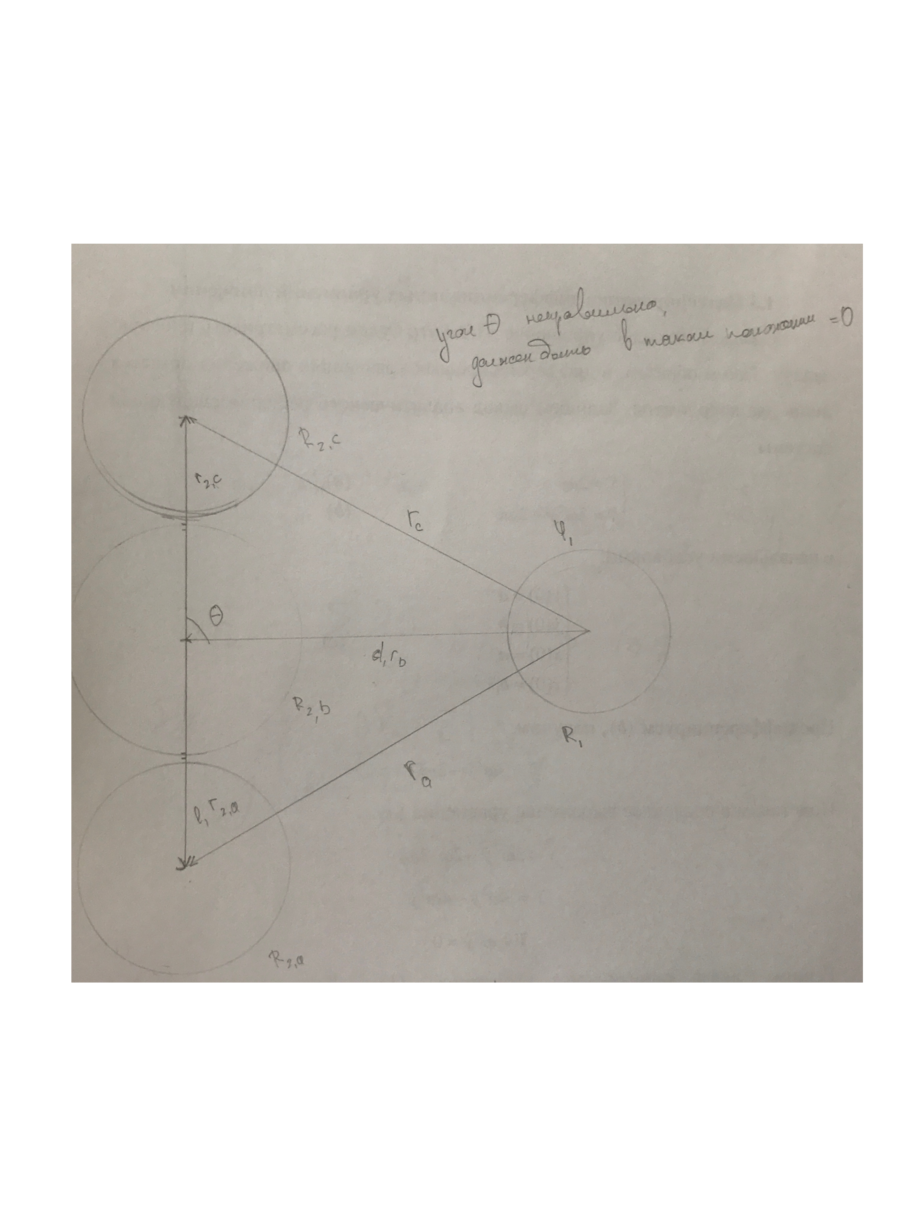
\includegraphics[scale=0.5]{3sph.png}}
	\caption{Замена космического аппарата сферами}
	\label{ris:3sph}
\end{figure} 

Для моделирования взаимодействия между космическими аппаратами нужно решить матричное уравнение относительно вектора зарядов:
\begin{equation*}
\label{eq:3sph_q_eq}
	\begin{pmatrix}
		q_1\\
		q_{2a}\\
		q_{2b}\\
		q_{2c}
	\end{pmatrix}
	= k_c C_m 
	\begin{pmatrix}
		-\phi\\
		\phi\\
		\phi\\
		\phi
	\end{pmatrix},
\end{equation*}
где $q_i$ – заряды сфер, $\phi$ – абсолютное значение напряжения для любой из сфер (оно берется одинаковым), $C_m$ – матрица емкостей, обратная матрица к которой имеет вид:
\begin{equation*}
\label{eq:3sph_cm}
	[C_m]^{-1} = 
	\begin{pmatrix}
		1/R_1	&	1/r_a	&	1/r_b	&	1/r_c\\
		1/r_a	&	1/R_{2a}	&	1/l		&	1/2l\\
		1/r_b	&	1/l		&	1/R_{2b}	&	1/l\\
		1/r_c	&	1/2l		&	1/l		&	1/R_{2c}
	\end{pmatrix}.
\end{equation*}

Взяв за обобщенную координату угол $\theta$, запишем обобщенную силу:
\begin{equation*}
\label{eq:3sph_Qj}
	Q_\theta = \frac{\partial \vec{r}_{ba}}{\partial \theta(t)} \cdot F_{2a} + \frac{\partial \vec{r}_{bc}}{\partial \theta(t)} \cdot F_{2c},
\end{equation*}
где вектор $\vec{r}_{ba}$ – вектор между центрами сфер $A$ и $B$, $\vec{r}_{bc}$ – вектор между центрами сфер $B$ и $C$, $F_{2a}$ и $F_{2c}$ – силы электростатического взаимодействия в центре внешней сферы:
\begin{equation*}
\label{eq:3sph_F2a}
	F_{2a} = - \frac{k_c q_1 q_{2a}}{r_a^3} \vec{R}_a,
\end{equation*}
\begin{equation*}
\label{eq:3sph_F2c}
	F_{2c} = - \frac{k_c q_1 q_{2c}}{r_c^3} \vec{R}_c.
\end{equation*}

Так же, запишем кинетическую энергию:
\begin{equation*}
\label{eq:3sph_kin}
	T = \frac{J \left(\frac{d \theta (t)}{dt}\right)^2}{2},
\end{equation*}
где $J$ – момент инерции.

Имея это, решим уравнение Лагранжа второго рода при разных расстояниях $d$ для двух случаев: с фиксированными значениями зарядов для угла $\theta = 0$ и для зарядов, вычисленных по методу многих сфер. 

\begin{figure}[H]
	\center{\includegraphics[scale=0.4]{msm_theta_d=20.png}}
	\caption{Зависимость угла $\theta$ от времени $t$ для $d=20$м}
	\label{ris:3sph_theta_d=20}
\end{figure}

\begin{figure}[H]
	\center{\includegraphics[scale=0.4]{msm_theta_d=10.png}}
	\caption{Зависимость угла $\theta$ от времени $t$ для $d=10$м}
	\label{ris:3sph_theta_d=10}
\end{figure}

\begin{figure}[H]
	\center{\includegraphics[scale=0.4]{msm_theta_d=5.png}}
	\caption{Зависимость угла $\theta$ от времени $t$ для $d=5$м}
	\label{ris:3sph_theta_d=5}
\end{figure}

\begin{figure}[H]
	\center{\includegraphics[scale=0.4]{{msm_theta_d=1.8}.png}}
	\caption{Зависимость угла $\theta$ от времени $t$ для $d=1.8$м}
	\label{ris:3sph_theta_d=1.8}
\end{figure}

Как видно из рисунков \ref{ris:3sph_theta_d=20} - \ref{ris:3sph_theta_d=1.8} при уменьшении расстояния $d$ фиксированное произведение зарядов становится всё менее точным.
Отсюда можно сделать вывод, что метод многих сфер есть смысл применять при  сравнительно небольших расстояниях между объектами.



\section*{Заключение}

В данной работе проведено исследования системы из активного и пассивного космического аппаратов. Моделирование производилось с помощью программ для среды Wolfram Mathematica.

В главе 2 рассмотрено движение вокруг центра масс пассивного космического аппарата цилиндрической формы при постоянном расстоянии между центрами масс аппаратов. Моделирование проводилось с помощью метода многих сфер.

В главе 3 проведено моделирование взаимодействия космических аппаратов, представленных материальными точками, с приложением тяги к активному аппарату. Были составлены и проанализированы тяги управления.

В главе 4 рассмотрено движение вокруг центра масс пассивного космического аппарата цилиндрической формы в системе с активным космическим аппаратом. Было произведено исследование управляющей функции. Моделирование так же проводилось с помощью метода многих сфер. Так как моделирование производилось в бессиловом поле, полученная модель пригодна для расчетов подобных взаимодействий на большом удалении от притягивающего центра или в поле действия силы тяжести (моделирование на земле).
\end{document}